The conveyor belt layer has two tasks: feed a consistent stream of boxes to the arm, and comply with safety standards. This layer has two subsystems: The ON/OFF controller, which receives signals from the PLC to start or stop the conveyor belt, and the 'Box Ready' Photo Eyes signaling system, which uses photo eyes to detect when another box is ready to be picked up.

\subsection{Conveyor Belt Hardware}
A conveyor belt provided by the Senior Design labs.

\subsubsection{Conveyor Belt Programming Languages}
Python/URScript

\begin{figure}[h!]
\centering
 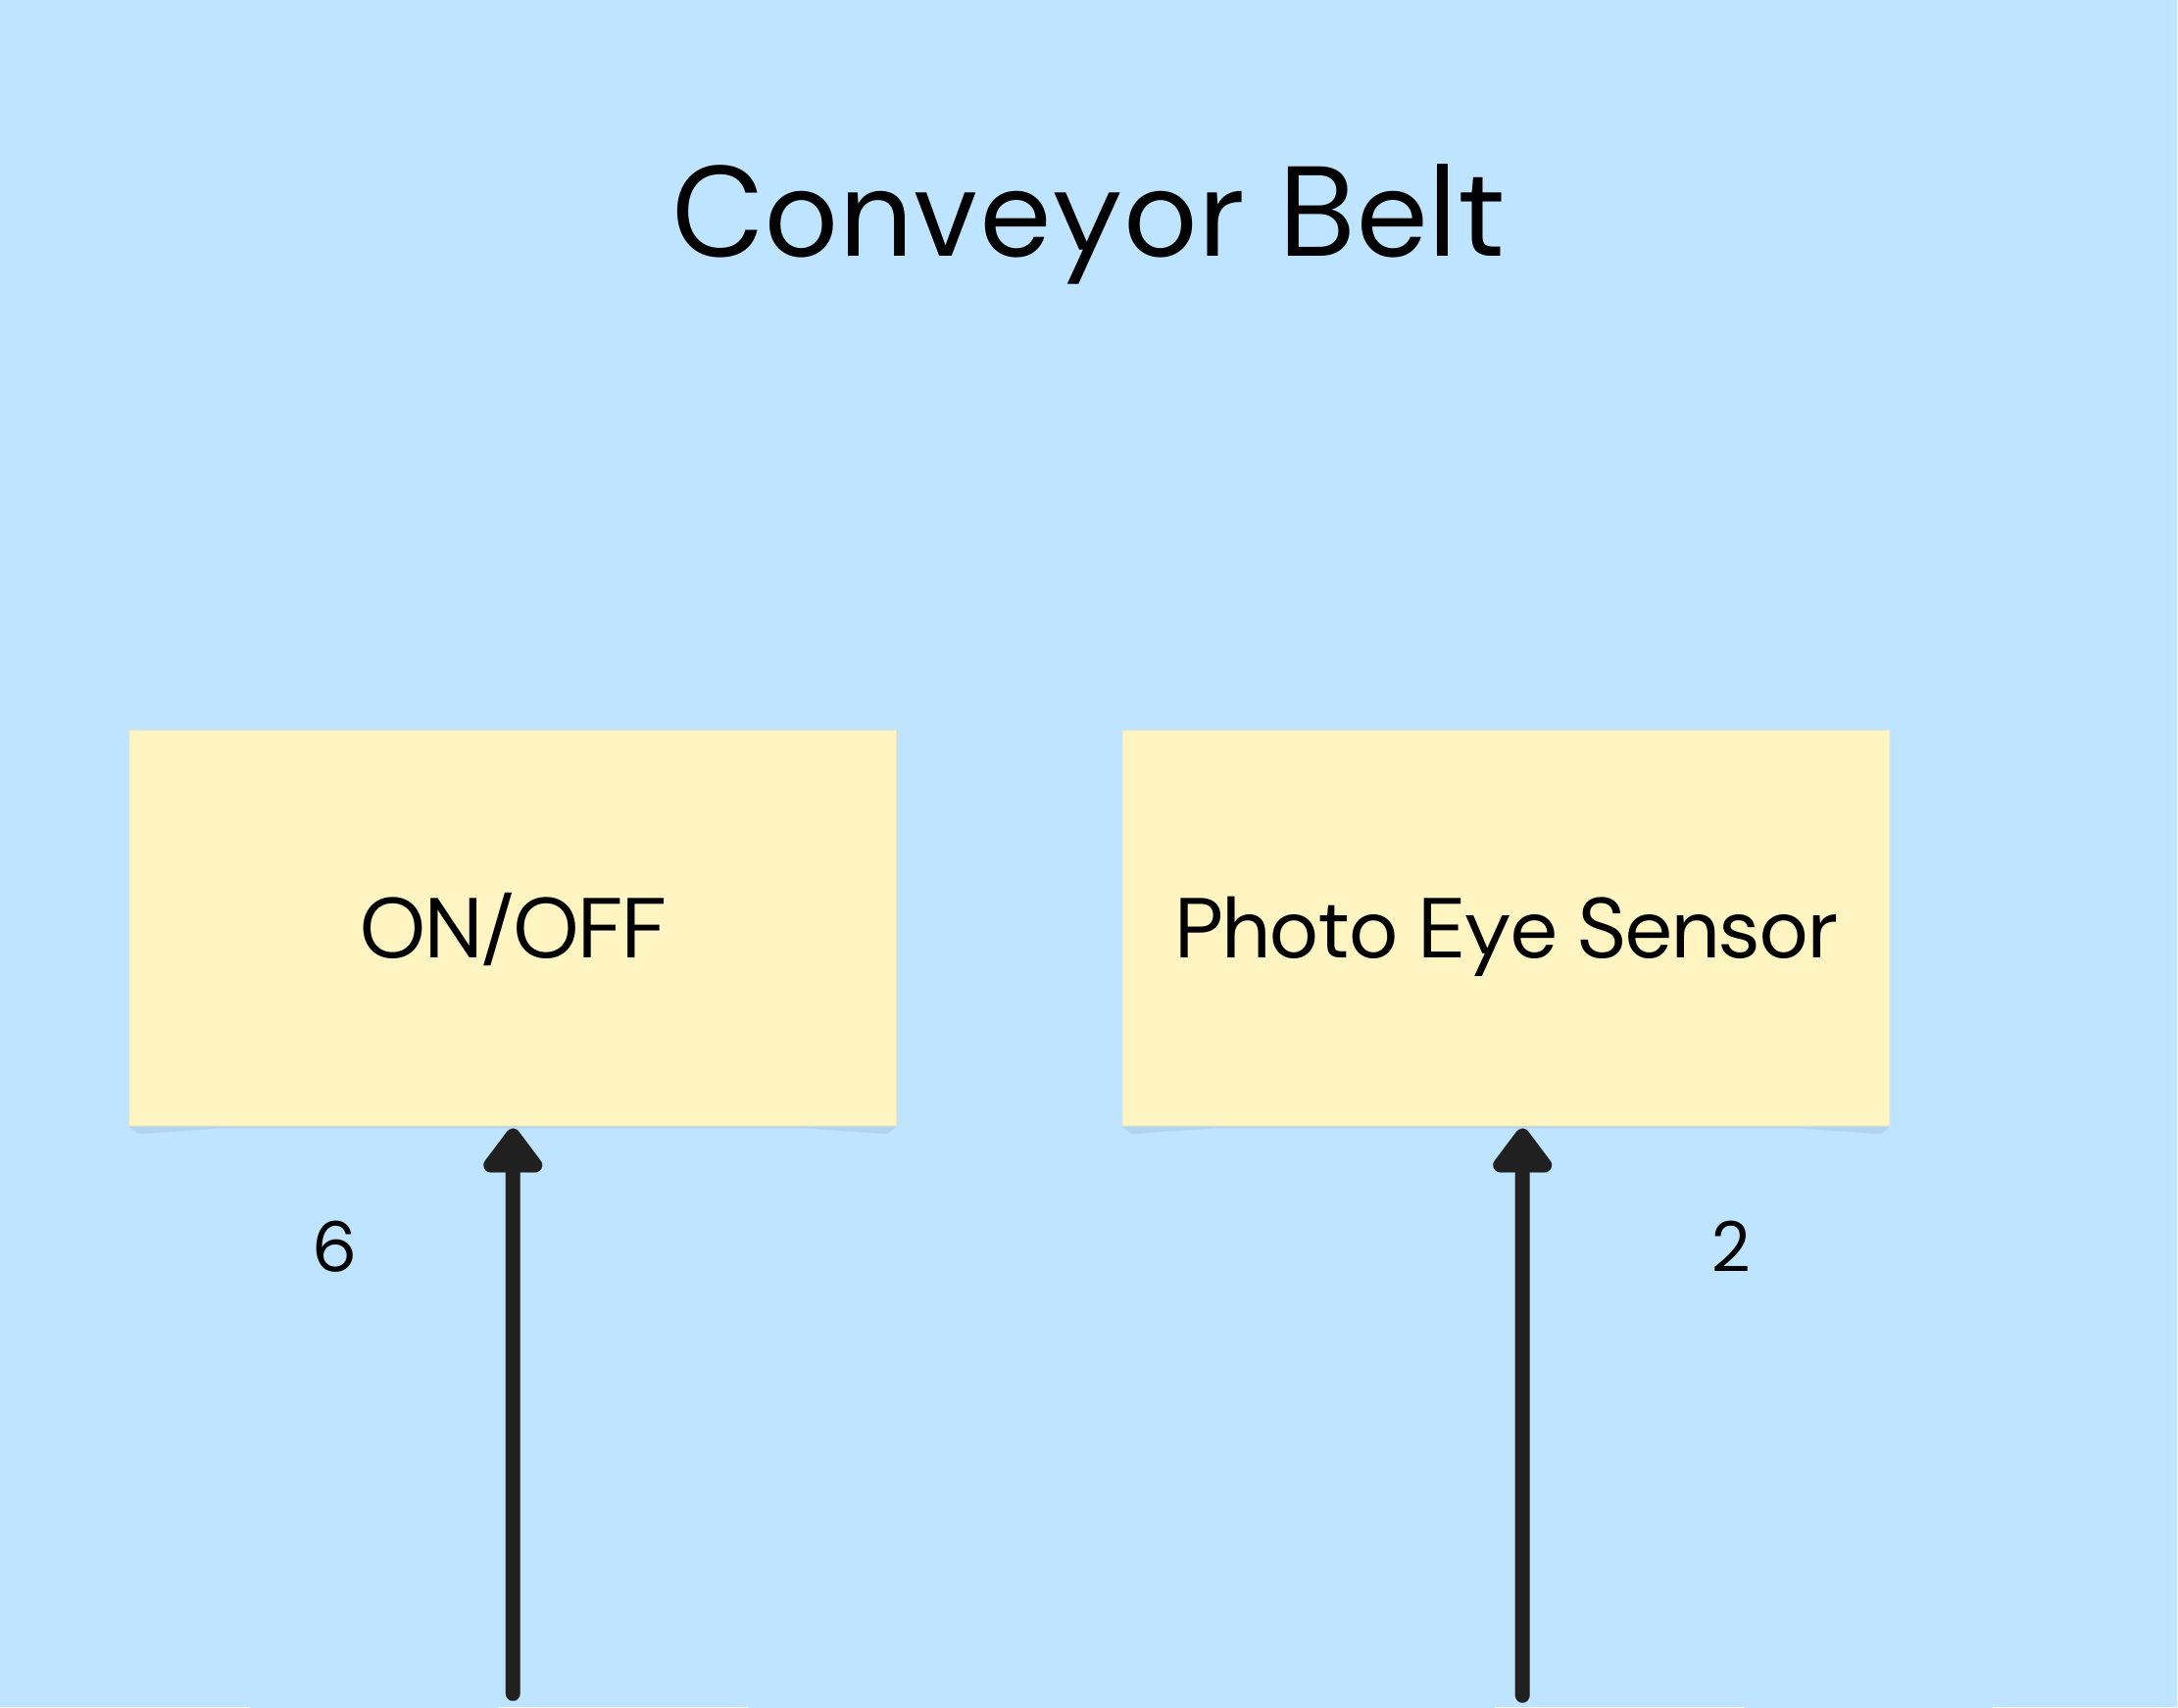
\includegraphics[width=0.60\textwidth]{images/conveyor.png}
 \caption{Conveyor belt diagram}
\end{figure}

\subsubsection{Conveyor Belt Software Dependencies}
URX Python library

\subsection{Power Controller Subsystem}
The power controller hardware subsystem in the conveyor belt layer is responsible for controlling the state of the conveyor belt. The subsystem receives a command from the PLC to switch the belt "ON" or "OFF" when operations begin or end, OR when the safety system indicates an emergency stop.

\subsubsection{Power Controller Hardware}
A power supply toggle for emergency shut-off, wired to the robot arm to be controlled by the PLA.

\subsubsection{Power Controller Data Structures}
This is a binary on/off toggle of the conveyor belt, so a single binary bit should be all that is necessary.

\subsection{Photo Eye Subsystem}
The photo eye is a simple hardware module positioned at the end of the conveyor belt to indicate that a box has passed and is ready to pick up. 

\subsubsection{Photo Eye Hardware}
Wiring between the Photo Eye and robot arm inputs.

\subsubsection{Photo Eye Data Structures}
The most common photo eye design signals use a single bit, active when presence is initially detected, and otherwise the bit signals as inactive.
